\documentclass[11pt,a4paper]{article}
\usepackage[margin=2.5cm]{geometry}
\usepackage{amsmath,amssymb,bm}
\usepackage{graphicx}
\usepackage{booktabs}
\usepackage{subcaption}
\usepackage{algorithm}
\usepackage{algpseudocode}
\usepackage{float}
\usepackage[font=small,labelfont=bf]{caption}
\usepackage{cite}
\usepackage{hyperref}
\hypersetup{colorlinks=true,linkcolor=black,citecolor=black,urlcolor=black}
% continue the numbering of the main report (Section 6, Eq. 28, Fig. 11, Table 7, Alg. 2)
\setcounter{section}{6}
\setcounter{equation}{28}
\setcounter{figure}{11}
\setcounter{table}{7}
\setcounter{algorithm}{2}
\begin{document}



% =====================================================================
%  Section: High-Dimensional Application, ANN Training
%  Insert with \input{ann_section} after Section 6 (before Future Plans).
%  Needs: amsmath, amssymb, booktabs, graphicx, subcaption,
%         algorithm, algpseudocode (all already used in the report).
%  Placeholders: values in bold square brackets [ ... ] and framed
%  boxes for figures. Search for "\ph{" and "\figph{" to find them.
% =====================================================================
\providecommand{\ph}[1]{\textbf{[#1]}}
\providecommand{\figph}[2]{\fbox{\parbox[c][#1][c]{0.94\linewidth}{\centering\small\textit{Figure placeholder:}\\[2pt] #2}}}

\section{High-Dimensional Application: ANN Training}
\label{sec:ann}

\subsection{Motivation}
\label{sec:ann:motivation}
The benchmarks in Sections 3 to 5 have at most 100 design variables and a known global minimum. They are well suited for following the path of the optimizer, but practical problems in engineering and machine learning usually have thousands to millions of unknowns. In this section, we will explore the training of an ANN (Artificial Neural Network) with respect to different ADAM variants.

Even the moderate network used for the 100-dimensional problem below, with layer widths $[100, 128, 64, 1]$, has
\begin{equation}
  P = \sum_{l=1}^{L} n_l\,(n_{l-1}+1) = 12\,928 + 8\,256 + 65 = 21\,249
\end{equation}
trainable parameters. The gradient with respect to all of them is obtained with the adjoint method (backpropagation) at a cost comparable to one forward pass. A central finite-difference approximation would need $2P = 42\,498$ forward passes per gradient. In addition, the loss of a neural network has no single known minimizer. Performance is measured by how well the trained model predicts data it has not seen, which is a different criterion from the distance to $w^*$ used in Section 5.

\subsection{Network Model}
\label{sec:ann:model}
The network maps an input $\bm{x}\in\mathbb{R}^{n_0}$ to an output $\bm{y}\in\mathbb{R}^{n_L}$ through $L$ fully connected layers with widths $[n_0, n_1, \dots, n_L]$. Each layer has a weight matrix $\bm{W}^{(l)}\in\mathbb{R}^{n_l\times n_{l-1}}$ and a bias vector $\bm{b}^{(l)}\in\mathbb{R}^{n_l}$. The samples are stored column-wise, $\bm{X}=[\bm{x}_1,\dots,\bm{x}_N]$, so that one forward pass evaluates a whole batch:
\begin{align}
  \bm{A}^{(0)} &= \bm{X}, \\
  \bm{Z}^{(l)} &= \bm{W}^{(l)}\bm{A}^{(l-1)} + \bm{b}^{(l)}\mathbf{1}^{\mathsf T}, \qquad l = 1,\dots,L, \\
  \bm{A}^{(l)} &= \sigma\big(\bm{Z}^{(l)}\big) \quad (l<L), \qquad \bm{A}^{(L)} = \bm{Z}^{(L)} .
\end{align}
The hidden layers use the activation function $\sigma$ element-wise, and the output layer is linear. The training objective is the mean squared error over all outputs and all $N_b$ samples of the current batch,
\begin{equation}
  J(\bm{\theta}) = \frac{1}{n_L N_b}\,\big\| \bm{A}^{(L)} - \tilde{\bm{Y}} \big\|_F^2 ,
  \label{eq:ann:loss}
\end{equation}
where $\tilde{\bm{Y}}$ are the standardized targets (Section~\ref{sec:ann:data}) and $\bm{\theta}$ collects all weights and biases.

\begin{figure}[H]
  \centering
   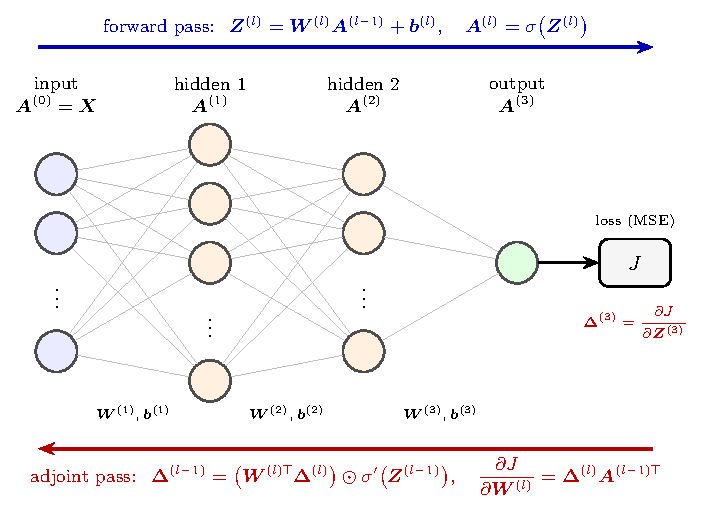
\includegraphics[width=0.85\textwidth]{figures/ANN/ann_schematic.pdf}
  \caption{Fully connected network with forward pass (left to right) and adjoint pass (right to left).}
  \label{fig:ann:schematic}
\end{figure}

\subsection{Gradient by the Adjoint Method}
\label{sec:ann:adjoint}
The gradient of $J$ is computed by reverse-mode differentiation, known in the neural network literature as backpropagation \cite{rumelhart1986learning} and in the optimization literature as the discrete adjoint method \cite{baydin2018automatic}. For each layer the adjoint variable is the sensitivity of the loss with respect to the pre-activation,
\begin{equation}
  \bm{\Delta}^{(l)} = \frac{\partial J}{\partial \bm{Z}^{(l)}} .
\end{equation}
It is initialised at the linear output layer by differentiating Eq.~\eqref{eq:ann:loss},
\begin{equation}
  \bm{\Delta}^{(L)} = \frac{2}{n_L N_b}\big(\bm{A}^{(L)} - \tilde{\bm{Y}}\big),
\end{equation}
and propagated backwards with
\begin{equation}
  \bm{\Delta}^{(l-1)} = \Big(\big(\bm{W}^{(l)}\big)^{\mathsf T}\bm{\Delta}^{(l)}\Big)\odot\sigma'\big(\bm{Z}^{(l-1)}\big), \qquad l = L,\dots,2 .
\end{equation}
The parameter gradients of every layer follow directly from the adjoint and the stored activations of the forward pass:
\begin{equation}
  \frac{\partial J}{\partial \bm{W}^{(l)}} = \bm{\Delta}^{(l)}\big(\bm{A}^{(l-1)}\big)^{\mathsf T},
  \qquad
  \frac{\partial J}{\partial \bm{b}^{(l)}} = \bm{\Delta}^{(l)}\mathbf{1}.
\end{equation}
One backward pass costs a small multiple of one forward pass, independent of $P$. The gradients are returned in a structure with the same fields as the parameters ($\bm{W}^{(1)},\bm{b}^{(1)},\dots$), so they can be passed directly to the same optimizer step functions used in the previous sections.

\subsection{Gradient check against central finite differences}
To verify the adjoint gradient, it was compared with central finite differences on a small network ($[1,5,4,1]$, $\tanh$, 20 random samples). Every weight and bias $\theta_j$ is perturbed by $\pm h$:
\begin{equation}
  g_j^{\mathrm{FD}} = \frac{J(\bm{\theta}+h\bm{e}_j) - J(\bm{\theta}-h\bm{e}_j)}{2h}, \qquad h=10^{-6},
\end{equation}
and the relative error $|g_j^{\mathrm{FD}} - g_j^{\mathrm{adj}}| / \max(1,|g_j^{\mathrm{FD}}|)$ is computed. The largest error over all parameters was 2.44 $\times 10^{-9}$, well below the threshold of $10^{-5}$, so the adjoint implementation is correct.

\begin{table}[H]
  \centering
  \caption{Gradient check: maximum relative error between adjoint and central finite-difference gradients (layers $[1,5,4,1]$, $\tanh$, $h=10^{-6}$).}
  \label{tab:ann:gradcheck}
  \begin{tabular}{lccc}
    \toprule
    \textbf{Parameter array} & \textbf{Size} & \textbf{Max. relative error $e$} & \textbf{Passed ($e<10^{-5}$)} \\
    \midrule
    $\bm{W}^{(1)}$ & $5\times1$ & 1.27 $\times10^{-9}$ & yes \\
    $\bm{b}^{(1)}$ & $5\times1$ & 2.44 $\times10^{-9}$ & yes \\
    $\bm{W}^{(2)}$ & $4\times5$ & 1.94 $\times10^{-9}$ & yes \\
    $\bm{b}^{(2)}$ & $4\times1$ & 1.25 $\times10^{-9}$ & yes \\
    $\bm{W}^{(3)}$ & $1\times4$ & 3.07 $\times10^{-10}$ & yes \\
    $\bm{b}^{(3)}$ & $1\times1$ & 3.03 $\times10^{-11}$ & yes \\
    \bottomrule
  \end{tabular}
\end{table}

\subsection{Training Setup}
\label{sec:ann:data}
\paragraph{Data.} The samples are split randomly into 70\% training, 15\% validation and 15\% test data. Inputs are scaled to $[-1,1]$ and outputs are standardized, using training statistics only. A scaled MSE of 1 therefore means the model is no better than predicting the mean. After each epoch the validation loss is computed, the weights with the lowest validation loss are kept, and the test set is used once at the end.

\paragraph{Batch size.} The batch size $B$ sets how many samples are used per gradient and update. With $B = N_{\mathrm{tr}}$ the method is full-batch gradient descent (one update per epoch, exact gradient), with $1 < B < N_{\mathrm{tr}}$ it is mini-batch training, and with $B = 1$ it is stochastic gradient descent (SGD). The samples are shuffled every epoch. The results below use full batch.

\paragraph{Optimizers and fairness.} ADAM, AdamW \cite{loshchilov2017decoupled}, AMSGrad \cite{reddi2018convergence} and Twin ADAM (Section 6.4) are compared using the same training code, only the step function is exchanged. For Twin ADAM two networks are trained on the same data and coupled as in Section 6.4, which costs two gradients per update. All runs use the same random seed, so data, split and initial weights are identical, and the same hyperparameters (Table~\ref{tab:ann:setup}).

\begin{table}[H]
  \centering
  \caption{Test problems and common settings.}
  \label{tab:ann:setup}
  \begin{tabular}{lp{0.72\textwidth}}
    \toprule
    \textbf{Test problems} & Rosenbrock fit with $D = 1$, $2$, $100$ inputs; real-world data set Concrete Compressive Strength (UCI) \\
    \textbf{Network (100D)} & $[100, 128, 64, 1]$, $P = 21\,249$, $N = 100\,000$ samples in $[-2,2]^{100}$ \\
    \textbf{Activation} & $\tanh$ (hidden), linear (output) \\
    \textbf{Hyperparameters} & $\alpha = 0.01$, $\beta_1 = 0.9$, $\beta_2 = 0.999$, $\varepsilon = 10^{-8}$, AdamW $\lambda = 0.1$ \\
    \textbf{Batch size} & full batch ($B = N_{\mathrm{tr}}$) \\
    \textbf{Seed} & 1, reset before every run \\
    \bottomrule
  \end{tabular}
\end{table}

\begin{algorithm}[H]
\caption{ANN training with an exchangeable ADAM-type optimizer (\texttt{ADAM\_ANN.m})}
\label{alg:ann}
\begin{algorithmic}[1]
\Require Data $(\bm{X},\bm{Y})$, layer widths, activation $\sigma$, epochs $E$, batch size $B$, step function \texttt{opt}, hyperparameters $(\alpha,\beta_1,\beta_2,\varepsilon)$
\State Split data 70/15/15; scale inputs to $[-1,1]$, standardize outputs (training statistics)
\State Initialise $\bm{\theta}$; optimizer state $\leftarrow\emptyset$; $t\leftarrow0$; $J^{\mathrm{best}}_{\mathrm{va}}\leftarrow\infty$
\For{$e = 1,\dots,E$}
  \State Shuffle the training samples
  \For{each batch $\mathcal{B}$ of size $B$}
    \State $\bm{A}^{(L)} \leftarrow$ forward pass on $\mathcal{B}$ \Comment{store $\bm{Z}^{(l)},\bm{A}^{(l)}$}
    \State $\nabla_{\bm{\theta}} J \leftarrow$ adjoint pass on $\mathcal{B}$ \Comment{Section~\ref{sec:ann:adjoint}}
    \State $t\leftarrow t+1$
    \State $[\bm{\theta},\text{state}] \leftarrow \texttt{opt}(\bm{\theta},\nabla_{\bm{\theta}}J,\text{state},t,\text{hp})$ \Comment{ADAM, AdamW, AMSGrad}
  \EndFor
  \State Evaluate $J_{\mathrm{tr}}$ and $J_{\mathrm{va}}$ on the complete sets
  \If{$J_{\mathrm{va}} < J^{\mathrm{best}}_{\mathrm{va}}$}
    \State $J^{\mathrm{best}}_{\mathrm{va}}\leftarrow J_{\mathrm{va}}$; \ $\bm{\theta}^{\mathrm{best}}\leftarrow\bm{\theta}$
  \EndIf
\EndFor
\State Evaluate $J_{\mathrm{te}}$ with $\bm{\theta}^{\mathrm{best}}$
\State \Return $\bm{\theta}^{\mathrm{best}}$, loss histories, $J_{\mathrm{te}}$
\end{algorithmic}
\end{algorithm}



\paragraph{Evaluation criteria.}
Since the minimum of the training loss is unknown, the optimizers are compared by the quality of the trained model and the cost of training:
\begin{itemize}
  \item \textbf{Test MSE (scaled)} with the best-validation parameters. This is the main criterion, since it measures prediction on data not used in training.
  \item \textbf{Training MSE and best validation MSE}, to show how well the data is fitted.
  \item \textbf{Generalisation ratio} $G = J_{\mathrm{te}}/J_{\mathrm{tr}}$. Values close to 1 mean the model generalises; values much larger than 1 indicate overfitting.
  \item \textbf{Cost}: wall-clock time and the number of gradient evaluations. With $E$ epochs this is
\begin{equation}
  C \approx 6\,P\,k\,E\,N_{\mathrm{tr}},
\end{equation}
with $k=1$ for ADAM, AdamW and AMSGrad and $k=2$ for Twin ADAM. With the same $P$, $E$ and $N_{\mathrm{tr}}$ for all optimizers, Twin ADAM therefore has twice the cost of the other methods, which is consistent with the measured times.
\end{itemize}

\subsection{Twin ADAM for Network Training}
\label{sec:ann:twin}
The twin-gradient step-length modulation of Section 6.4 \cite{demagistris2026twin} was transferred to the network. Two networks with independent random initialisations, $\bm{\theta}_1$ and $\bm{\theta}_2$, are trained on the same batches. Both compute their own ADAM step $\bm{s}_1,\bm{s}_2$, and the multipliers $\gamma_1,\gamma_2$ are obtained from the same $2\times2$ system as in Section 6.4, with all weights and biases of a network treated as one vector:
\begin{equation}
  \min_{\gamma_1,\gamma_2}\ \big\| (\bm{\theta}_1 + \gamma_1\bm{s}_1) - (\bm{\theta}_2 + \gamma_2\bm{s}_2) \big\|_2^2 ,
  \qquad \gamma_{1,2}\in[0.5,\,3.5].
\end{equation}
If the two steps are nearly parallel the system is close to singular, and $\gamma_1=\gamma_2=1$ is used, which reduces to two independent ADAM runs. After each epoch both networks are evaluated on the validation set, and the better one is kept as the current best model. Each update needs one forward and one adjoint pass for each network, i.e.\ two gradient evaluations instead of one.




\subsection{Results}
\label{sec:ann:results}
Table~\ref{tab:ann:results} summarises all ANN benchmarks.

\begin{table}[H]
  \centering
  \caption{ANN benchmark results (scaled MSE, seed 1, settings of Table~\ref{tab:ann:setup}).}
  \label{tab:ann:results}
  \small
  \begin{tabular}{lcccccc}
    \toprule
    \textbf{Optimizer} & \textbf{Train MSE} & \textbf{Best val.\ MSE} & \textbf{Test MSE} & \textbf{$G$} & \textbf{Time [s]}  \\
    \midrule
    \multicolumn{6}{l}{\textit{sin(0.2x) + 0.05*randn(1,200) }} \\
    ADAM      & $4.67\times10^{-3}$ & $1.32\times10^{-2}$ & $1.20\times10^{-2}$ & $2.56$ & $2.99$ \\
    AdamW     & $1.64\times10^{-1}$ & $1.15\times10^{-1}$ & $1.18\times10^{-1}$ & $0.72$ & $3.80$ \\
    AMSGrad   & $2.34\times10^{-1}$ & $3.24\times10^{-1}$ & $3.19\times10^{-1}$ & $1.37$ & $3.91$ \\
    Twin ADAM & $9.42\times10^{-3}$ & $1.36\times10^{-2}$ & $1.30\times10^{-2}$ & $1.38$ & $6.99$ \\
    \midrule
    \multicolumn{6}{l}{\textit{Rosenbrock 2D}} \\
    ADAM      & 5.16 $\times10^{-5}$ & 1.48 $\times10^{-4}$ & 4.70 $\times10^{-5}$ & 0.91 & 1.99  \\
    AdamW     & 2.21 $\times10^{-3}$ & 5.04 $\times10^{-3}$ & 2.54 $\times10^{-3}$ & 1.14 & 1.98  \\
    AMSGrad   & 1.02 $\times10^{-4}$ & 3.07 $\times10^{-4}$ & 9.36 $\times10^{-5}$ & 0.92 & 1.95 \\
    Twin ADAM & 8.31 $\times10^{-5}$ & 2.50 $\times10^{-4}$ & 8.39 $\times10^{-5}$ & 1.0 & 3.2  \\
    \midrule
    \multicolumn{6}{l}{\textit{Rosenbrock 100D}} \\
    ADAM      & 2.01 $\times10^{-1}$ & 5.44 $\times10^{-1}$ & 5.44 $\times10^{-1}$ & 2.70 & 493.18  \\
    AdamW     & 2.95 $\times10^{-1}$ & 6.27 $\times10^{-1}$ & 6.44 $\times10^{-1}$ & 2.18 & 531.00  \\
    AMSGrad   & 1.94 $\times10^{-1}$ & 5.26 $\times10^{-1}$ & 5.23 $\times10^{-1}$ & 2.69 & 573.19 \\
    Twin ADAM & 5.21 $\times10^{-1}$ & 7.12 $\times10^{-1}$ & 7.25 $\times10^{-1}$ & 1.39 & 950.16 \\
    \midrule
    \multicolumn{6}{l}{\textit{Real-world data set: Concrete dataset}} \\
    ADAM      & 4.68 $\times10^{-2}$ & 9.23 $\times10^{-2}$ & 1.15 $\times10^{-1}$ & 2.46  & 3.37  \\
    AdamW     & 4.20 $\times10^{-2}$ & 7.61 $\times10^{-2}$ & 1.13 $\times10^{-1}$ & 2.71  & 3.34\\
    AMSGrad   & 8.51 $\times10^{-2}$ & 1.05 $\times10^{-1}$ & 1.42 $\times10^{-1}$ & 1.67 & 3.56   \\
    Twin ADAM & 4.83 $\times10^{-2}$ & 7.48 $\times10^{-2}$ & 1.53 $\times10^{-1}$ & 3.17 & 6.04  \\
    \bottomrule
  \end{tabular}
\end{table}

\subsubsection{Low-dimensional Curve fits ($D=1$, $D=2$)}
Figure~\ref{fig:ann:lowdim} compares the learned function with the exact sin(0.2x) function with 0.5\% noise. The prediction follows the exact curve with a scaled test MSE of \ph{value}. For the 2D Rosenbrock the prediction reproduces the curved valley. These two cases show that the complete pipeline works before it is applied in high dimension. The differences between the optimizers are \ph{small / large}, see Table~\ref{tab:ann:results}.

\begin{figure}[H]
  \centering
  \begin{subfigure}[t]{0.62\textwidth}
    \centering
   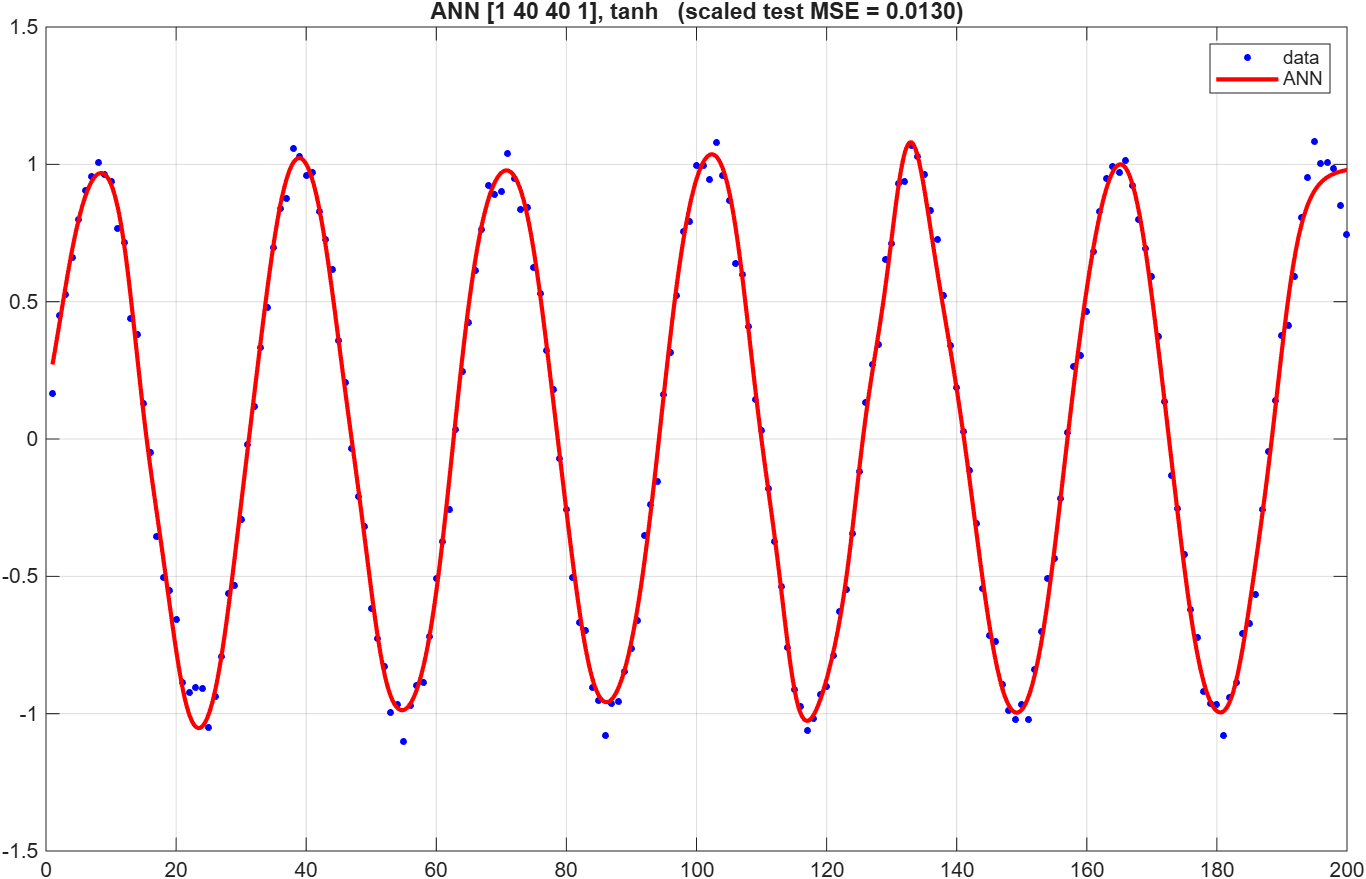
\includegraphics[width=\textwidth]{figures/ANN/1d_curve_fitting}
  \end{subfigure}
  \caption{ANN approximation of the for a 1D function sin(0.2x) with 0.5\% noise (ADAM, settings of Table~\ref{tab:ann:setup}).}
  \label{fig:ann:lowdim}
\end{figure}

\begin{figure}[H]
  \centering
  \begin{subfigure}[t]{0.48\textwidth}
    \centering
   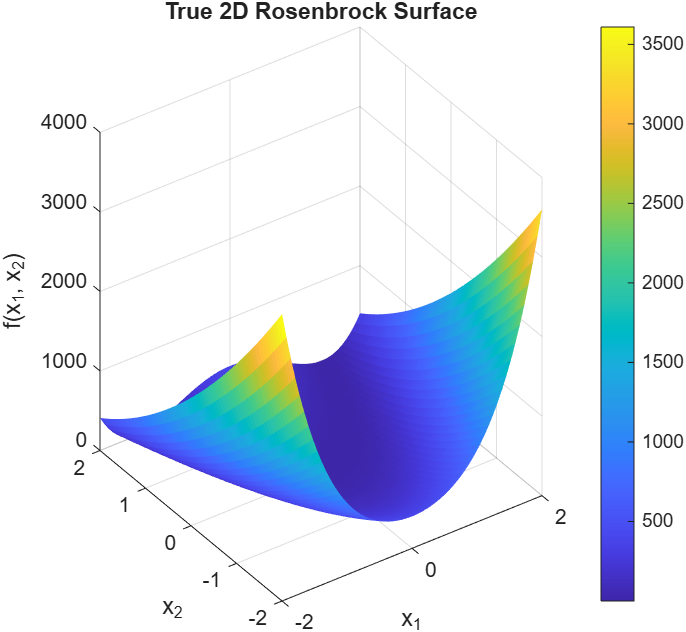
\includegraphics[width=\textwidth]{figures/ANN/2d_real_function.png}
    \caption{Original Function}
  \end{subfigure}\hfill
  \begin{subfigure}[t]{0.48\textwidth}
    \centering
   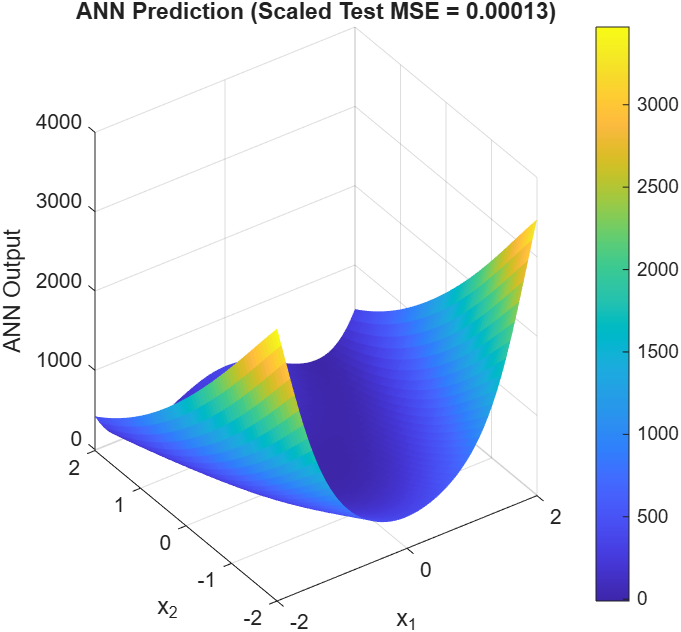
\includegraphics[width=\textwidth]{figures/ANN/2d_ANN_pred.png}
    \caption{ANN prediction}
  \end{subfigure}
  \caption{ANN approximation of the 2D Rosenbrock function (ADAM, settings of Table~\ref{tab:ann:setup}).}
  \label{fig:ann:rosen2d}
\end{figure}

\subsubsection{100-dimensional Rosenbrock ($D=100$, $P=21\,249$)}
Figure~\ref{fig:ann:conv100} shows the validation and training loss of the four optimizers over the epochs. \ph{Describe the curves: which optimizer decreases fastest in the first epochs, which one reaches the lowest validation loss, whether any curve stagnates or oscillates.} The lowest test MSE was obtained by \ph{optimizer} with \ph{value}. The generalisation ratio was between \ph{min} and \ph{max} for all optimizers, which \ph{does / does not} indicate overfitting with $N = 100\,000$ samples. Figure~\ref{fig:ann:parity} compares predicted and true values on the test set.

\begin{figure}[H]
  \centering
  \begin{subfigure}[t]{0.48\textwidth}
    \centering
   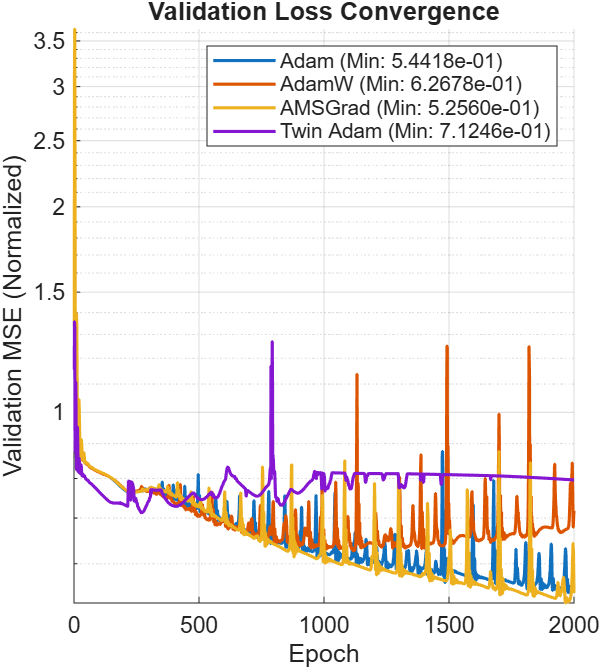
\includegraphics[width=\textwidth]{figures/ANN/100d_val_MSE.png}
    \caption{Validation loss}
  \end{subfigure}\hfill
  \begin{subfigure}[t]{0.48\textwidth}
    \centering
   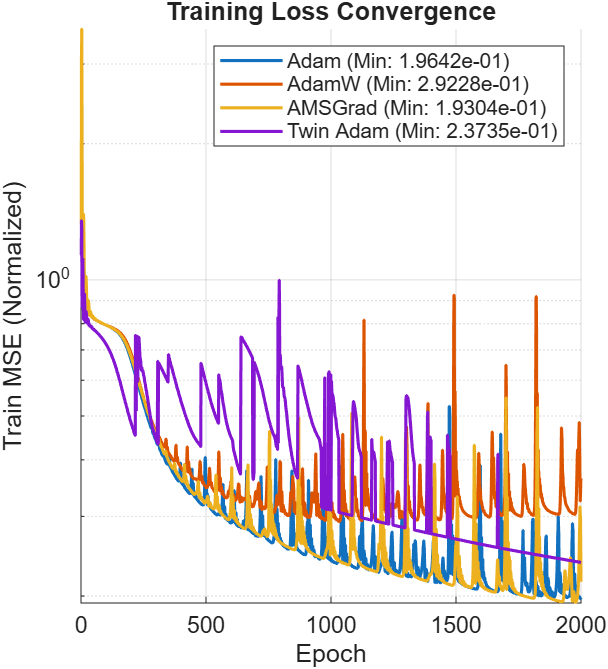
\includegraphics[width=\textwidth]{figures/ANN/100d_train_MSE.png}
    \caption{Training loss}
  \end{subfigure}
  \caption{Convergence of ADAM, AdamW, AMSGrad and Twin ADAM for the 100-dimensional Rosenbrock regression.}
  \label{fig:ann:conv100}
\end{figure}




\subsubsection{Real-world data set.} 
As a test on measured data, the Concrete Compressive Strength data set from the UCI Machine Learning Repository was used \cite{yeh1998concrete}. It contains 1030 laboratory tests without missing values. Each sample has 8 inputs: the amounts of cement, blast furnace slag, fly ash, water, superplasticizer, coarse aggregate and fine aggregate (all in kg/m$^3$ of mixture) and the age of the concrete in days. The output is the compressive strength in MPa. The relation between mixture and strength is strongly nonlinear, which is why the data set was originally used to test neural networks \cite{yeh1998concrete}. Unlike the Rosenbrock fits, the data contain measurement scatter, and with $N=1030$ the training set (721 samples) is small compared to the number of network parameters, so overfitting becomes possible. The same split, scaling and settings as for the other problems were used. \ph{Results: test MSE of the optimizers, Table~\ref{tab:ann:results}, and Figure~\ref{fig:ann:real}.}

\begin{figure}[H]
  \centering
   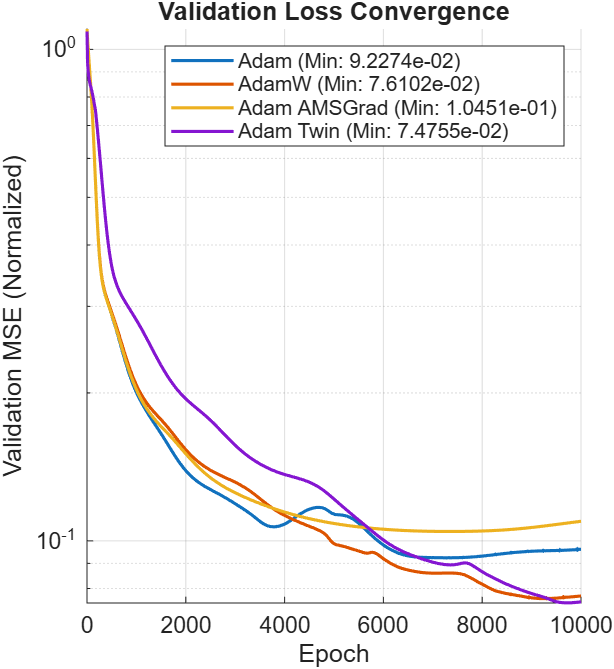
\includegraphics[width=0.5\textwidth]{figures/ANN/concrete_val_epoch_comp.png}
  \caption{Validation loss of ADAM, AdamW, AMSGrad and Twin ADAM over the epochs for the Concrete Compressive Strength data set.}
  \label{fig:ann:real}
\end{figure}

\subsubsection{Twin ADAM}
In the ANN benchmarks Twin ADAM did not reach a lower validation loss than ADAM within the same number of epochs \ph{confirm with final numbers}. Since it computes two gradients per update, its wall time per epoch was \ph{x} times that of ADAM (Figure~\ref{fig:ann:twin}). This differs from the direct 100-dimensional Rosenbrock problem (Section 6.4), where the twin coupling could help when the learning rate was chosen too small.

A likely reason is the structure of the network loss. The hidden neurons of a layer can be permuted, together with their weights, without changing the output of the network. The loss therefore has many equivalent minima at different locations in parameter space. Two independently initialised networks generally move towards different ones of these minima, so the direction that brings $\bm{\theta}_1$ and $\bm{\theta}_2$ closer together is not a direction that reduces the loss. The step multipliers then mainly act as a change of the learning rate. On problems with a single basin, such as the Rosenbrock function itself, the distance between the two iterates carries information about the position of the minimum, which is the situation the method was designed for \cite{demagistris2026twin}.

\begin{figure}[H]
  \centering
   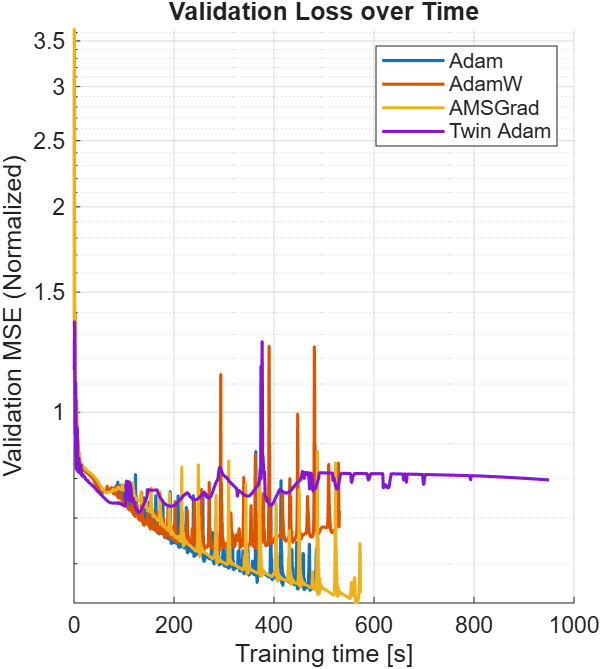
\includegraphics[width=0.5\textwidth]{figures/ANN/100d_val_MSE_time.png}
  \caption{ADAM and Twin ADAM compared at equal computing time (100-dimensional Rosenbrock regression).}
  \label{fig:ann:twin}
\end{figure}

\subsection{Discussion}
\label{sec:ann:discussion}
The ANN experiments extend the benchmarks of Sections 3 to 6 from at most 100 to 21\,249 unknowns. The adjoint method gave gradients that agreed with central finite differences to \ph{order of $e$}, at the cost of one backward pass instead of $2P$ loss evaluations. \ph{Summarise the main ranking of ADAM, AdamW and AMSGrad over the test problems in one or two sentences, and whether the ranking from the direct Rosenbrock problem in Section 5.4 carries over to network training.} Twin ADAM doubled the cost per update without improving the result on the networks, while it can help on the single-basin problems of Section 6.4.

All runs use one fixed seed and the same hyperparameters, so the comparison isolates the effect of the update rule. Repeated runs with other seeds and a study of the learning rate would show how sensitive the ranking is to these choices.

\bibliographystyle{plain}
\bibliography{references}

\end{document}